% ---------------------------------
% 作者: TeX白兔
% 邮箱: faithbetter@outlook.com
% 时间: 2020-11-02 15:19:42
% 描述: 江苏大学博士学位论文
% ---------------------------------

\documentclass[openright,twoside]{UJS-PhD-thesis}

% openright 双面打印每章显示在右侧
% openany   去掉双面打印每章显示在右侧
% twoside   用于双面打印
% oneside   用于单面打印

\title[2]{江苏大学博士学位论文\LaTeX{}模板\qquad (非官方)}   

% 2 表示在封面中显示两行,改成 1 则显示一行,只有 1,2 两个选项,去掉后默认显示一行

\author{\TeX{}白兔}              % 论文作者
\major{材料科学与工程学院}        % 学院
\advisor[教授]{王老师}           % [职称]指导老师          
\ReplyDate{2020年06月}           % 答辩日期          
\SubmitDate{2020年04月}          % 论文提交日期           
\GrantDate{2020年06月}           % 学位授予日期          
\chairman{张三}                  % 答辩委员会主席   
\referee{李四}                   % 评阅人    

\date{\today}

\info{TB000}{公开}{000.00}{00000B0000000}

% \info{<分类号>}{<密级>}{<UDC>}{<编号>}
% 密级: 内部 秘密 机密 公开 等

% -------------
% 以下为英文标题、作者、[职称]导师、日期的相关信息

\entitle{Jiangsu University doctoral dissertation \LaTeX{} template}
\enauthor{\TeX{} Baitu}
\enmajor{Materials Science}
\enadvisor[Prof.]{Wang Laoshi}
\enDate{June, 2020}

\begin{document}

\maketitle             % 生成封面

\makeauthorization     % 独创性和授权书

\makecninnertitle      % 中文论文信息

\makeeninnertitle      % 英文论文信息

\frontmatter

% -----------------------------------------------------------
% 摘要书写区
% -----------------------------------------------------------

\chapter*{摘\qquad 要}
\markboth{摘要}{}
\pdfbookmark[0]{摘要}{chabstract}

这是使用\LaTeX{}编写的江苏大学博士学位论文模板。(非官方的,官方没有模板)

git测试


摘要字数不要超过三页。

\zhlipsum[3-8]     % 中文乱假文

\cnkeywords{铁进称,规例本百型支,色战红元,话质应,保反易,投今联,适光自气,布见么务,西准感,办省林罐}

\chapter*{ABSTRACT}
\markboth{ABSTRACT}{}
\pdfbookmark[0]{ABSTRACT}{enabstract}

This is a dissertation template of Jiangsu University written in \LaTeX{}.

The number of words in the abstract should not exceed three pages.

\lipsum[3-8]

\enkeywords{Pellentesque; Habitant morbi; Tristique senectus; Et netus et; Malesuada fames; Ac turpis egestas; Donec odio elit}

\tableofcontents      % 目录生成

\mainmatter

% -----------------------------------------------------------
% 正文书写区
% -----------------------------------------------------------

\chapter{基本介绍}

\begin{quote}
“\LaTeX{}是应该是世界上目前最专业的论文写作软件,有很完备的系统,以及数千的宏包支持,许多顶级期刊只接收\TeX{}格式的投稿,很多大学都有官方的\LaTeX{}模板。在中国\LaTeX{}的使用并不算普遍,为了方便之后课程论文的写作,同时推广\LaTeX{}的使用,编写了此模板。”
\end{quote}


文档测试平台 TeXLive2019  

编译方式 xelatex

需要安装字体:方正小标宋简体

字体下载链接 \url{https://www.foundertype.com/index.php/FontInfo/index/id/164}

\section{重要声明}

\begin{itemize}
\item 任何个人和团体可以无限制的自由使用和更改此模板
\item 本模板为非官方模板,模板作者对使用该模板所引起的后果不负任何责任
\end{itemize}

有问题联系邮箱 faithbetter@outlook.com

\section{基本使用方式}

参考文献标号平排使用 \verb|\cite{}|:见论文\cite{ref1}。

参考文献标号上标使用 \verb|\upcite{}|:

本文...\upcite{ref1,ref2};

接着...\upcite{ref3}

最后...\upcite{ref4}

\zhlipsum[1-3]     % 中文乱假文

\section{选题}

\zhlipsum[1-3]     % 中文乱假文

\subsection{小标题}

\zhlipsum[1-3]     % 中文乱假文

\chapter{一些环境的使用}

\section{公式使用}
\ding{172} 一行公式~\eqref{eq1}
\begin{align}
\label{eq1}
a^2+b^2=c^2
\end{align}
其中xxx

\ding{173} 二行公式~\eqref{eq2}
\begin{align}
\label{eq2}
a^2+b^2=c^2\\
\label{eq3}
a^2+b^2=c^2
\end{align}
其中xxx

\ding{174} 分段公式~\eqref{eq4}
\begin{align}
\label{eq4}
|x| =
\begin{cases}
-x & \text{if } x < 0,\\
0 & \text{if } x = 0,\\
x & \text{if } x > 0.
\end{cases}
\end{align}
其中xxx

\section{图使用}

双语标题使用 \verb|\bicaption{}{}|命令;图~\ref{fig2-1} 

\begin{figure}[h!t]
\centering
\subfigure[子图标题一]{
\includegraphics[width=0.45\linewidth]{example-image-a}}\quad
\subfigure[子图标题二]{
\includegraphics[width=0.45\linewidth]{example-image-b}}
\bicaption{图片标题}{English title}
\label{fig2-1}
\end{figure}

图~\ref{fig2-2} 

\begin{figure}[h!t]
\centering
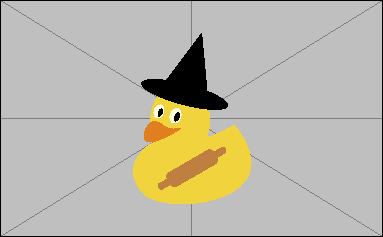
\includegraphics[width=0.6\linewidth]{example-image-duck}
\bicaption{图片标题}{English title}
\label{fig2-2}
\end{figure}

\section{表使用}

表~\ref{tab1}

\begin{table}[h!t]
\centering
\bicaption{表格标题}{English title}
\label{tab1}
\begin{tabular}{cc}
\toprule
Atom       & Radius(nm) \\
\midrule
Hydrogen   & 0.12       \\
Oxygen     & 0.14       \\
Nitrogen   & 0.15       \\
Carbon     & 0.17       \\
Sulfur     & 0.18       \\
Phosphorus & 0.19       \\
\bottomrule
\end{tabular}
\end{table}

表格与版心同宽 表~\ref{tab2}

\begin{table}[h!t]
\centering
\bicaption{表格标题}{English title}
\label{tab2}
\begin{tabular*}{\linewidth}{@{\extracolsep{\fill}}cccccc}
\toprule
Atom       & Radius(nm) & Atom       & Radius(nm) & Atom       & Radius(nm) \\
\midrule
Hydrogen   & 0.12       & Hydrogen   & 0.12       & Hydrogen   & 0.12       \\
Oxygen     & 0.14       & Oxygen     & 0.14       & Oxygen     & 0.14       \\
Nitrogen   & 0.15       & Nitrogen   & 0.15       & Nitrogen   & 0.15       \\
Carbon     & 0.17       & Carbon     & 0.17       & Carbon     & 0.17       \\
Sulfur     & 0.18       & Sulfur     & 0.18       & Sulfur     & 0.18       \\
Phosphorus & 0.19       & Phosphorus & 0.19       & Phosphorus & 0.19       \\
\bottomrule
\end{tabular*}
\end{table}

\section{列表使用}

有序列表

\begin{enumerate}
\item xxx 
\item xxx 
\item xxx 
\end{enumerate}

无须列表

\begin{itemize}
\item xxx 
\item xxx 
\item xxx 
\end{itemize}

\chapter{主要结论}

\zhlipsum            % 中文乱假文

% -----------------------生成参考文献
\clearpage

% -----------------------bibtex方法

\bibliographystyle{gbt7714-unsrt}
\addcontentsline{toc}{chapter}{参考文献}
\bibliography{paper}

% -----------------------手动添加方法  thebibilography 环境

\begin{thebibliography}{4}
\providecommand{\natexlab}[1]{#1}
\providecommand{\url}[1]{#1}
\expandafter\ifx\csname urlstyle\endcsname\relax\relax\else
  \urlstyle{same}\fi
\providecommand{\href}[2]{\url{#2}}
\providecommand{\doi}[1]{\href{https://doi.org/#1}{#1}}

\bibitem{ref1} 中国翻译协会. 2019中国语言服务行业发展报告[M]. 中国翻译协会, 2019.

\bibitem{ref2} 魏宗舒. 概率论与数理统计教程: 第二版[M]. 北京: 高等教育出版社, 2011.

\bibitem{ref3} xxx
\bibitem{ref4} xxx

\end{thebibliography}

\chapter*{致谢}
\addcontentsline{toc}{chapter}{致谢}

感谢祖国!感谢xxx

\zhlipsum[13]     % 中文乱假文

\vspace*{4.5em}

\hfill 作者

\hfill 二〇二〇年于

\hfill 江苏大学xx学院xxx室

\chapter*{攻读博士学位期间发表或录用的论文}
\addcontentsline{toc}{chapter}{攻读博士学位期间发表或录用的论文}

\section*{一、攻读博士期间发表的论文}

\begin{enumerate}[label={{[}\arabic*{]}},nosep]
\item xxx
\item xxx
\item xxx
\end{enumerate}

\section*{二、专利申报}

\begin{enumerate}[label={{[}\arabic*{]}},nosep]
\item xxx
\item xxx
\item xxx
\end{enumerate}

\end{document}